
\vspace{2mm}
\noindent \textbf{Estimation of the exit probability.} We consider \eqref{eq:OneDModel} with $D = \left[ -1, 1 \right]$, the final time $T = 1$, initial condition $X_0 = 0$ and we define
\begin{align}\label{eq:FunctionsOneDSmoothPhi}
\begin{split}
	f(x) &= -V'(x), \text{ where } V(x) = 0.1(8x^4 - 8x^2 + x + 2), \\
	g(x) &= \sigma = 2.
\end{split}
\end{align}
In order to approximate $\Phi$, we perform a Montecarlo simulation using both DEM and CEM, with $M = 10^5$ trajectories. We consider the number of timesteps for the time integration to be $N = 2^i, i = 3, \dots, 9$. The reference solution used to compute errors is obtained with Finite Differences applied to problem \eqref{eq:PDEPhi} (see Appendix \ref{sec:Appendix2}). Numerical results (Figure \ref{fig:KillOneDPhi}) confirm that the weak error for DEM is of order 0.5. For CEM it is not trivial to show a clear order of convergence one. This is due to the fact that the results are accurate already with a big step size, therefore the statistical error is not negligible with respect to the error due to time integration. In order to avoid the noise on the order of convergence, it would be necessary to increase the number of trajectories dramatically, leading to unaffordable computational times. Let us remark that CEM approximates the exit probability better than DEM for any initial value $X_0$, as shown in Figure \ref{fig:PhiProfiles}.

\begin{figure}[t]
    \centering
    \begin{subfigure}{0.49\linewidth}
        \centering
        \resizebox{1\linewidth}{!}{% This file was created by matlab2tikz.
%
%The latest updates can be retrieved from
%  http://www.mathworks.com/matlabcentral/fileexchange/22022-matlab2tikz-matlab2tikz
%where you can also make suggestions and rate matlab2tikz.
%
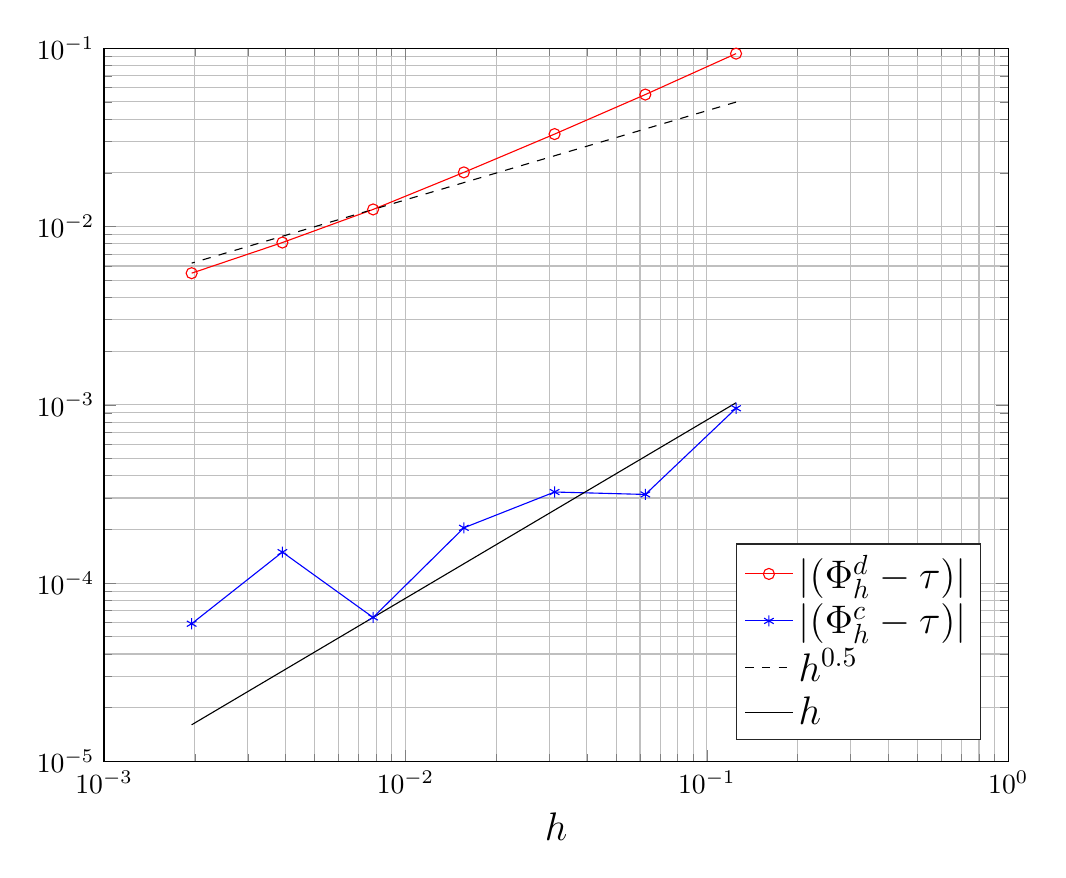
\begin{tikzpicture}

\begin{axis}[%
width=4.521in,
height=3.566in,
at={(0.758in,0.481in)},
scale only axis,
xmode=log,
xmin=0.001,
xmax=1,
xminorticks=true,
xlabel={$h$},
xlabel style={font=\Large},
xmajorgrids,
xminorgrids,
ymode=log,
ymin=1e-05,
ymax=0.1,
yminorticks=true,
ymajorgrids,
yminorgrids,
axis background/.style={fill=white},
legend pos = south east,
legend style={legend cell align=left,align=left,draw=white!15!black,font=\Large}
]
\addplot [color=red,solid,mark=o,mark options={solid}]
  table[row sep=crcr]{%
0.125	0.0931958331986392\\
0.0625	0.0549308331986392\\
0.03125	0.0329758331986393\\
0.015625	0.0201058331986392\\
0.0078125	0.0124608331986392\\
0.00390625	0.00812583319863924\\
0.001953125	0.00547083319863928\\
};
\addlegendentry{$|\E(\Phi_h^d - \tau)|$};

\addplot [color=blue,solid,mark=asterisk,mark options={solid}]
  table[row sep=crcr]{%
0.125	0.000955833198639233\\
0.0625	0.00031416680136076\\
0.03125	0.000324166801360715\\
0.015625	0.000204166801360706\\
0.0078125	6.41668013607877e-05\\
0.00390625	0.000149166801360789\\
0.001953125	5.91668013607549e-05\\
};
\addlegendentry{$|\E(\Phi_h^c - \tau)|$};

\addplot [color=black,dashed]
  table[row sep=crcr]{%
0.125	0.0498433327945569\\
0.0625	0.035244558615969\\
0.03125	0.0249216663972784\\
0.015625	0.0176222793079845\\
0.0078125	0.0124608331986392\\
0.00390625	0.00881113965399225\\
0.001953125	0.00623041659931961\\
};
\addlegendentry{$h^{0.5}$};

\addplot [color=black,solid]
  table[row sep=crcr]{%
0.125	0.0010266688217726\\
0.0625	0.000513334410886301\\
0.03125	0.000256667205443151\\
0.015625	0.000128333602721575\\
0.0078125	6.41668013607877e-05\\
0.00390625	3.20834006803938e-05\\
0.001953125	1.60417003401969e-05\\
};
\addlegendentry{$h$};

\end{axis}
\end{tikzpicture}%
 }  
        \caption{Killing boundary in $x = 1$}
        \label{fig:KillOneDPhi}
    \end{subfigure}
    \begin{subfigure}{0.49\linewidth}
        \centering
        \resizebox{1\linewidth}{!}{% This file was created by matlab2tikz.
%
%The latest updates can be retrieved from
%  http://www.mathworks.com/matlabcentral/fileexchange/22022-matlab2tikz-matlab2tikz
%where you can also make suggestions and rate matlab2tikz.
%
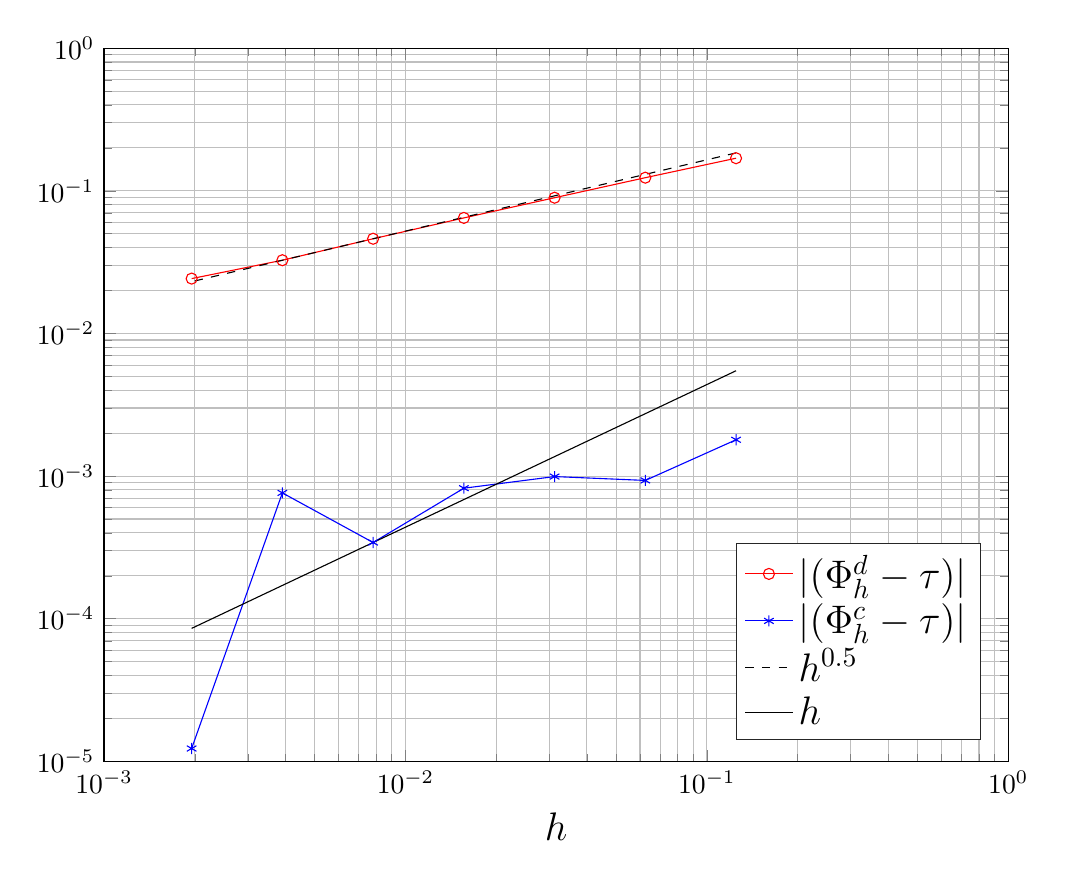
\begin{tikzpicture}

\begin{axis}[%
width=4.521in,
height=3.566in,
at={(0.758in,0.481in)},
scale only axis,
xmode=log,
xmin=0.001,
xmax=1,
xminorticks=true,
xlabel={$h$},
xlabel style = {font=\Large},
xmajorgrids,
xminorgrids,
ymode=log,
ymin=1e-05,
ymax=1,
yminorticks=true,
ymajorgrids,
yminorgrids,
axis background/.style={fill=white},
legend pos = south east,
legend style={legend cell align=left,align=left,draw=white!15!black,font=\Large}
]
\addplot [color=red,solid,mark=o,mark options={solid}]
  table[row sep=crcr]{%
0.125	0.169237691826179\\
0.0625	0.123577691826179\\
0.03125	0.0894376918261789\\
0.015625	0.0645576918261789\\
0.0078125	0.0461076918261789\\
0.00390625	0.032607691826179\\
0.001953125	0.024237691826179\\
};
\addlegendentry{$|\E(\Phi_h^d - \tau)|$};

\addplot [color=blue,solid,mark=asterisk,mark options={solid}]
  table[row sep=crcr]{%
0.125	0.00179769182617895\\
0.0625	0.000932308173821061\\
0.03125	0.000992308173821121\\
0.015625	0.000822308173821118\\
0.0078125	0.000342308173821082\\
0.00390625	0.000762308173821058\\
0.001953125	1.23081738211406e-05\\
};
\addlegendentry{$|\E(\Phi_h^c - \tau)|$};

\addplot [color=black,dashed]
  table[row sep=crcr]{%
0.125	0.184430767304716\\
0.0625	0.130412246220603\\
0.03125	0.0922153836523578\\
0.015625	0.0652061231103013\\
0.0078125	0.0461076918261789\\
0.00390625	0.0326030615551507\\
0.001953125	0.0230538459130895\\
};
\addlegendentry{$h^{0.5}$};

\addplot [color=black,solid]
  table[row sep=crcr]{%
0.125	0.00547693078113731\\
0.0625	0.00273846539056866\\
0.03125	0.00136923269528433\\
0.015625	0.000684616347642164\\
0.0078125	0.000342308173821082\\
0.00390625	0.000171154086910541\\
0.001953125	8.55770434552705e-05\\
};
\addlegendentry{$h$};

\end{axis}
\end{tikzpicture}%
 }  
        \caption{Reflecting boundary in $x = 1$}
        \label{fig:ReflectOneDPhi}
    \end{subfigure}    
    \caption{Approximation of $\Phi$. Orders of convergence of DEM and CEM in the one-dimensional case.}
    \label{fig:OrdersOneDPhi}
\end{figure}

\begin{figure}[t]
    \centering
    \begin{subfigure}{0.49\linewidth}
        \centering
        \resizebox{1\linewidth}{!}{% This file was created by matlab2tikz.
%
%The latest updates can be retrieved from
%  http://www.mathworks.com/matlabcentral/fileexchange/22022-matlab2tikz-matlab2tikz
%where you can also make suggestions and rate matlab2tikz.
%
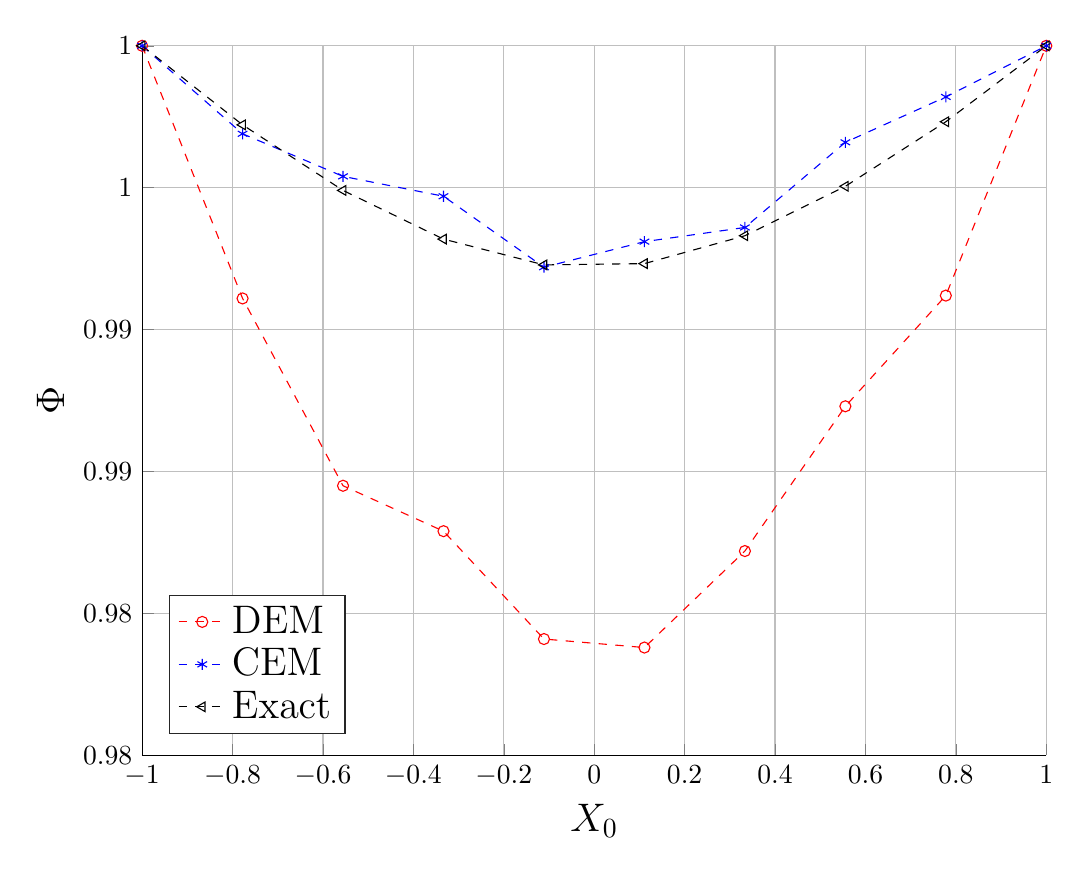
\begin{tikzpicture}

\begin{axis}[%
width=4.521in,
height=3.548in,
at={(0.758in,0.499in)},
scale only axis,
xmin=-1,
xmax=1,
xlabel={$X_0$},
xlabel style={font=\Large},
xmajorgrids,
ymin=0.975,
ymax=1,
ylabel={$\Phi$},
ylabel style={font=\Large},
ymajorgrids,
axis background/.style={fill=white},
axis x line*=bottom,
axis y line*=left,
legend style={at={(0.03,0.03)},anchor=south west,legend cell align=left,align=left,draw=white!15!black,font=\Large}
]
\addplot [color=red,dashed,mark=o,mark options={solid}]
  table[row sep=crcr]{%
-1	1\\
-0.777777777777778	0.9911\\
-0.555555555555556	0.9845\\
-0.333333333333333	0.9829\\
-0.111111111111111	0.9791\\
0.111111111111111	0.9788\\
0.333333333333333	0.9822\\
0.555555555555556	0.9873\\
0.777777777777778	0.9912\\
1	1\\
};
\addlegendentry{DEM};

\addplot [color=blue,dashed,mark=asterisk,mark options={solid}]
  table[row sep=crcr]{%
-1	1\\
-0.777777777777778	0.9969\\
-0.555555555555556	0.9954\\
-0.333333333333333	0.9947\\
-0.111111111111111	0.9922\\
0.111111111111111	0.9931\\
0.333333333333333	0.9936\\
0.555555555555556	0.9966\\
0.777777777777778	0.9982\\
1	1\\
};
\addlegendentry{CEM};

\addplot [color=black,dashed,mark=triangle,mark options={solid,rotate=90}]
  table[row sep=crcr]{%
-1	1\\
-0.777777777777778	0.99721538712255\\
-0.555555555555556	0.9949049913465\\
-0.333333333333333	0.993189956945965\\
-0.111111111111111	0.992280836629584\\
0.111111111111111	0.992326354174843\\
0.333333333333333	0.993308817442632\\
0.555555555555556	0.99505043807726\\
0.777777777777778	0.997324464142556\\
1	1\\
};
\addlegendentry{Exact};

\end{axis}
\end{tikzpicture}%
 }  
        \caption{Killing boundary in $x = 1$}
        \label{fig:KillPhiProfiles}
    \end{subfigure}
    \begin{subfigure}{0.49\linewidth}
        \centering
        \resizebox{1\linewidth}{!}{% This file was created by matlab2tikz.
%
%The latest updates can be retrieved from
%  http://www.mathworks.com/matlabcentral/fileexchange/22022-matlab2tikz-matlab2tikz
%where you can also make suggestions and rate matlab2tikz.
%
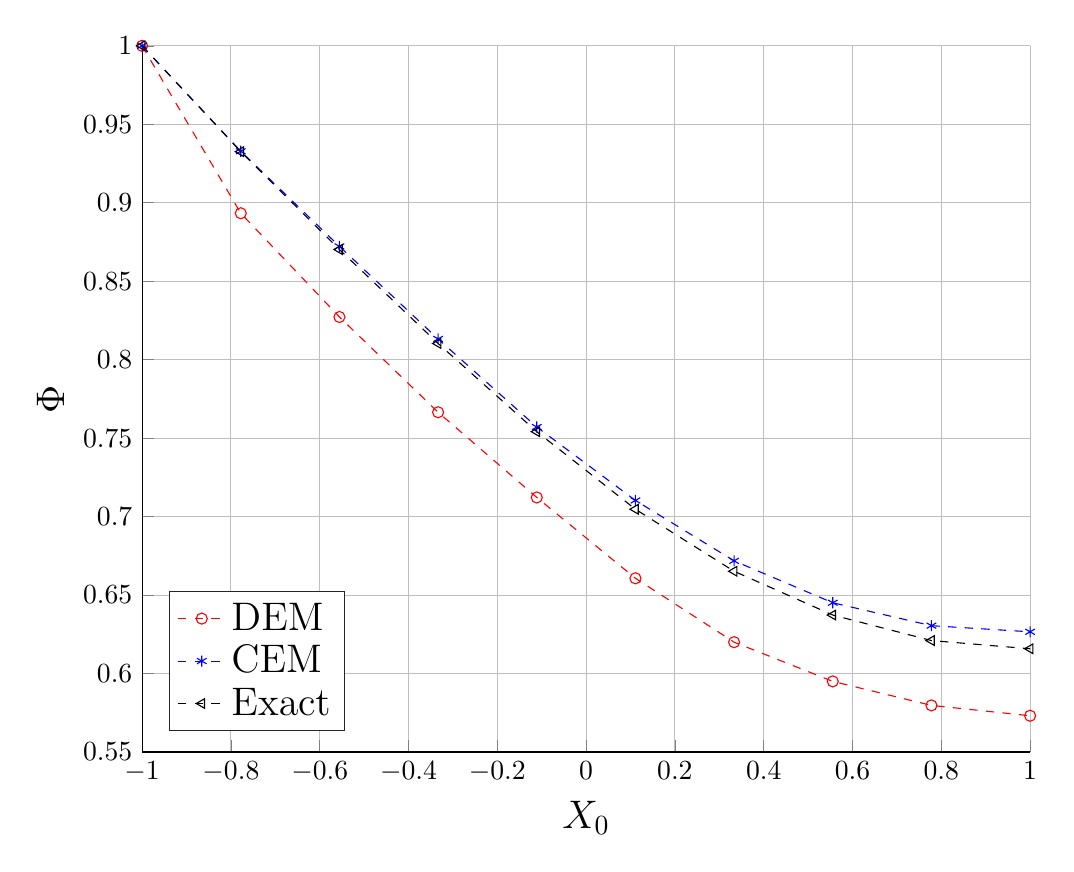
\begin{tikzpicture}

\begin{axis}[%
width=4.44in,
height=3.531in,
at={(0.745in,0.496in)},
scale only axis,
xmin=-1,
xmax=1,
xlabel={$X_0$},
xlabel style={font=\Large},
xmajorgrids,
ymin=0.55,
ymax=1,
ylabel={$\Phi$},
ylabel style={font=\Large},
ymajorgrids,
axis background/.style={fill=white},
axis x line*=bottom,
axis y line*=left,
legend style={at={(0.03,0.03)},anchor=south west,legend cell align=left,align=left,draw=white!15!black,font = \Large}
]
\addplot [color=red,dashed,mark=o,mark options={solid}]
  table[row sep=crcr]{%
-1	1\\
-0.777777777777778	0.8933\\
-0.555555555555556	0.8272\\
-0.333333333333333	0.7665\\
-0.111111111111111	0.7122\\
0.111111111111111	0.6607\\
0.333333333333333	0.62\\
0.555555555555556	0.595\\
0.777777777777778	0.5797\\
1	0.5731\\
};
\addlegendentry{DEM};

\addplot [color=blue,dashed,mark=asterisk,mark options={solid}]
  table[row sep=crcr]{%
-1	1\\
-0.777777777777778	0.9328\\
-0.555555555555556	0.8722\\
-0.333333333333333	0.8132\\
-0.111111111111111	0.7571\\
0.111111111111111	0.7103\\
0.333333333333333	0.6718\\
0.555555555555556	0.6451\\
0.777777777777778	0.6305\\
1	0.6266\\
};
\addlegendentry{CEM};

\addplot [color=black,dashed,mark=triangle,mark options={solid,rotate=90}]
  table[row sep=crcr]{%
-1	1\\
-0.777777777777778	0.932548077502788\\
-0.555555555555556	0.870181977112059\\
-0.333333333333333	0.810303153980793\\
-0.111111111111111	0.754108688988762\\
0.111111111111111	0.70469446885863\\
0.333333333333333	0.665180416423286\\
0.555555555555556	0.63727357440893\\
0.777777777777778	0.621019342130665\\
1	0.615785886384429\\
};
\addlegendentry{Exact};

\end{axis}
\end{tikzpicture}%
 }  
        \caption{Reflecting boundary in $x = 1$}
        \label{fig:ReflectPhiProfiles}
    \end{subfigure}    
    \caption{Approximation of $\Phi$ as a function of the initial value $X_0$.}
    \label{fig:PhiProfiles}
\end{figure}


